%!TEX root = ./main.tex

\section{Online \emph{linear} covering with experts}	\label{sec:covering}

\paragraph{Benchmark relaxation for the algorithm.}
%
%Our first proposed algorithm solves online linear covering problems by creating linear combinations of the solutions proposed by $K$ experts in an online manner.
%Recall that we evaluate the performance of our algorithm with the \texttt{LIN-COMB} benchmark (formalized on \cref{fig:benchmark}), which consists of the best linear combination of the experts' solution at each time step.

Since our \texttt{LIN-COMB} benchmark is a linear combination of the experts' solutions, the equality $ \sum_{k=1}^{K} w_{k}^{t} = 1$ must hold, where $w_{k}^{t} \geq 0$ is the weight assigned to expert $k$ at time~$t$. In the following, we formulate a relaxed version of \texttt{LIN-COMB}, where
$\sum_{k=1}^{K} w_{k}^{t} \geq 1$. The relaxed formulation also enables us to avoid the (online) hard constraint requiring $w_{k}^{t} s_{i,k}^{t} \geq w_{k}^{t-1} s_{i,k}^{t-1}$ to hold. Instead, we introduce a new variable, $y_{i}^{t}$, to represent the increase of $x_{i}^{t}$ compared to $x_{i}^{t-1}$. When $w_{k}^{t} s_{i,k}^{t} < w_{k}^{t-1} s_{i,k}^{t-1}$ during the execution, we set the contribution of $i$ at time $t$ to be 0, and therefore, $y_{i}^{t} = 0$.
The relaxed formulation of \texttt{LIN-COMB} is visible on Figure~\ref{fig:relaxation}.

\begin{figure}
	\begin{mdframed}
		\vspace{-0.2cm}
		\hspace{-0.5cm}
		\begin{minipage}[t]{6.5cm}
			\begin{align*}
					&& \min \sum_{t = 1}^{T} \sum_{i=1}^{n} & c_i y_i^t \\
					%
					&& \sum_{k=1}^{K} w_{k}^{t} & \geq 1  & \forall\ t \\
					%
					&& \sum_{k=1}^{K} \left(w_{k}^{t} s_{i,k}^{t} - w_{k}^{t-1} s_{i,k}^{t-1} \right) &\leq y_i^t  &\forall\ i,t\\
					%
					&& w_{k}^{t},\ y_{i}^{t} & \ge 0 & \forall\ i,t,k
				\end{align*}
		\end{minipage}
		\hspace{0.8cm}
		\begin{minipage}[t]{6cm}
			\begin{align*}
				&& \max \sum_{t=1}^{T} & \alpha^{t} \\
			%
				&& \alpha^{t} + \sum_{i=1}^{n} s_{i,k}^{t} ( \beta_{i}^{t+1} - \beta_{i}^{t})   &\leq 0  &\forall\ k,t\\
				%
				&& \beta_{i}^{t}   &\leq c_{i}  &\forall\ i,t \\
				%
				&& \alpha_{i}^{t},\ \beta_{i}^{t} & \ge 0 & \forall\ i,t
			\end{align*}
		\end{minipage}
	\end{mdframed}
	\caption{The relaxation of the \texttt{LIN-COMB} benchmark and its dual}
	\label{fig:relaxation}
\end{figure}

According to the theorem of weak duality, any feasible solution of the dual program lower bounds any feasible solution of the primal program, and therefore, any feasible dual solution also lower bounds our \texttt{LIN-COMB} benchmark. Following the chain of lower bounds, our approach to design a competitive algorithm is as follows. At every time step $t$, we build solutions for all $x_{i}^{t}$ together with the solutions for the dual problem $(\alpha^{t}, \beta_{i}^{t})$. Then, we bound the cost of the algorithm to that of the dual. It is important to emphasize that the designed solution for every $x_{i}^{t}$ must be feasible to the covering constraints, but it may \emph{not necessarily} be a linear combination of the experts' solutions.

\subsection{Algorithm description} \label{sec:algo}

\paragraph{Preprocessing.}
We recall that by our assumptions, the experts' solutions are always feasible and non-decreasing. At the arrival of the $t^{\text{th}}$ constraint, expert $k$ provides a feasible solution $s_{k}^{t} = (s_{i,k}^{t})_{i=1}^{n}$, such that $s_{i,k}^{t} \ge s_{i,k}^{t'}$ for all $t' \le t$ and all $i$. These assumptions do not exclude the possibility for the experts to provide malicious solutions that instruct the algorithm to use an unnecessarily large amount of resources.
Note that one difficulty of designing competitive algorithms comes from the lack of obvious ways to distinguish
good expert solutions from (probably many) non-efficient/misleading ones.

%To regardless maintain online solutions, we do \emph{not} expect the experts' solutions to be always tight (a difference compared to the assumptions in \cite{AnandGe22:Online-Algorithms}).
%(In Appendix~\ref{appix-tight-solutions}
%we show an example that tight solutions cannot be maintained in an online manner.)

To circumvent the issue of malicious suggestions, we preprocess the experts' solutions at each iteration. During the preprocessing, every solution $s_k^t$ is scaled down to make it as tight as possible on the $t^{\text{th}}$ constraint, while always maintaining $s_{i,k}^{t} \geq s_{i,k}^{t-1}$ for all $i$. Additionally, after the down-scaling, we create an auxiliary solution $\hat{s}_k^t$ that is tight for the $t^{\text{th}}$ constraint. An important highlight: this auxiliary solution is useful for our algorithm and its analysis, but it does \emph{not} directly participate in forming the actual solution. (Our algorithm only sets the weights of the experts and does not change the experts' solutions.) The auxiliary solution $\hat{s}_k^t$ is created with the following procedure.

After down-scaling the experts' suggestions, do the following for each expert $k$. $(1)$ If $(s_{i,k}^{t})_{i=1}^{n}$ is tight on the $t^{\text{th}}$ constraint, then for every~$i$ set $\hat{s}_{i,k}^{t}$ to $s_{i,k}^{t}$. $(2)$ Let $\hat{s}_{i,k}^{t-1}$ be the auxiliary solution of expert $k$ at time $t-1$, meaning that, $\sum_{i=1}^{n} a_{i}^{t-1} \hat{s}_{i,k}^{t-1} = 1$. Given $I := \{i: s_{i,k}^{t} > \hat{s}_{i,k}^{t-1} \cdot \sfrac{a_{i}^{t-1}}{a_{i}^{t}} \}$, if $i \notin I$ we set $\hat{s}_{i,k}^{t} \gets s_{i,k}^{t}$, and if $i \in I$, we set $\hat{s}_{i,k}^{t}$ to be some value in $[\hat{s}_{i,k}^{t-1} \cdot \sfrac{a_{i}^{t-1}}{a_{i}^{t}}, s_{i,k}^{t}]$ such that the solution $\hat{s}_{i,k}^{t}$ becomes tight on the $t^{\text{th}}$ constraint.

%\begin{restatable}{lemma}{preprocessinglemma}
%	\label{lem:preprocessing}
%	Following the preprocessing procedure, we can always obtain the solutions $\hat{s}_{i,k}^{t}$ such that
%	$\hat{s}_{i,k}^{t} \leq s_{i,k}^{t}$ and $\sum_{i=1}^{n} a_{i}^{t} \hat{s}_{i,k}^{t} = 1$.
%\end{restatable}
%For the proof of \cref{lem:preprocessing} see \cref{appix-proofs}.


%\paragraph{Algorithm.} The algorithm is visible on \cref{fig:algo1}.
%
\begin{figure}[ht]
\begin{mdframed}
\paragraph{\underline{Algorithm 1.}} At the arrival of the $t^{\text{th}}$ constraint

\vspace{0.1cm}
Step $(1)$: solve the following convex program and set $w^t$ to be the obtained optimal solution
%
\begin{align*}
	&& \min_{w} \biggl\{\sum_{i=1}^{n} c_{i}  \biggl[  \biggl(\sum_{k=1}^{K} s_{i,k}^{t} w_{i,k}  + \delta_{i}^{t} \biggr) &
	\ln \left( \frac{\sum_{k=1}^{K} s_{i,k}^{t} w_{i,k}  + \delta_{i}^{t}}{ \sum_{k=1}^{K}  s_{i,k}^{t-1}w_{i,k}^{t-1}  + \delta_{i}^{t-1}}  \right)
	- \sum_{k=1}^{K}  s_{i,k}^{t} w_{i,k} \biggr] \biggr\} \\
	%\end{align*}
	%%
	%\noindent subject to:
	%%
	%\begin{align*}
		(\gamma^{t})  && \sum_{i=1}^{n} a_{i}^{t} \biggl( \sum_{k=1}^{K}  \hat{s}_{i,k}^{t} w_{i,k} \biggr) &\geq 1 \qquad \forall\ t\\
		%
		(\lambda_{i}) && \sum_{k=1}^{K}  w_{i,k} &\geq 1 \qquad \forall\ i\\
		%
		(\mu_{i}^{t}) && \sum_{k=1}^{K} s_{i,k}^{t} w_{i,k} &\geq 0 \qquad \forall\ i,t
	\end{align*}
	%
	where $\delta_{i}^{t} = \frac{1}{K} \sum_{k} s_{i,k}^{t}$.
	%and recall that we set $\rho = \max_{i} \max_{t',t''} \left\{\frac{\sum_{k=1}^{K} s_{i,k}^{t'}}{\sum_{k=1}^{K} s_{i,k}^{t''}} : \sum_{k=1}^{K} s_{i,k}^{t''} > 0 \right\}$.
	We use the auxiliary solution $\hat{s}_{i,k}^{t}$ in the first constraint. For every $i$ where $s_{i,k}^{t} = 0$ for all $k$, the term related to $i$ is not included in the objective function ($w_{i,k} = 0$ for all $k$ beforehand).

	\vspace{0.1cm}
	Step $(2)$: For all $i$, if $\sum_{k} w_{i,k}^{t} s_{i,k}^{t} > x_{i}^{t-1}$ then set $x_{i}^{t} \gets \sum_{k} w_{i,k}^{t} s_{i,k}^{t}$;
	otherwise set $x_{i}^{t} \gets x_{i}^{t-1}$.
\end{mdframed}
	\caption{Algorithm 1 for online linear covering problems}
	\label{fig:algo1}
\end{figure}

\paragraph{Remark.} To set $(x_i^t)_{i=1}^n$ at each time $t$, our proposed algorithm solves an internal convex program, whose objective uses a shifted entropy function as a convex regularizer. To avoid a possible division by $0$, we use a dummy expert. This expert sets initially each variable to some small value, then follows the greedy heuristic at each arriving constraint. The presence of a dummy expert only changes the competitive ratio from $O(\log(K))$ to $O(\log(K + 1))$, so to simplify the notation, we display all other occurrences of the competitive ratio as $O(\log(K))$.
%At time $0$ (when no constraints have arrived yet), every expert's suggestion is $0$ for every variable, but the average of the suggestions is $1$.

\subsection{Performance Analysis}

\begin{theorem} \label{covering-theorem}
Algorithm 1 is $O(\ln(K \rho))$-competitive with the \texttt{LIN-COMB} benchmark.
\end{theorem}
%
\begin{proof} In \cref{appix:linear-proofs} we prove that Algorithm 1 creates feasible solutions for the dual problem of the \texttt{LIN-COMB} benchmark's relaxation and for the original covering problem. In the following we show that the algorithm's solution increases the primal objective value of the original covering problem by at most $O(\ln(K \rho))$ times the value of the relaxation's dual solution, which serves as the lower bound on the \texttt{LIN-COMB} benchmark.
	\begin{align}
		 \sum_{i=1}^{n} &c_{i} (x_{i}^{t} - x_{i}^{t-1})
			= \sum_{i: x_{i}^{t} > x_{i}^{t-1}} c_{i}(x_{i}^{t} - x_{i}^{t-1}) &&  \notag \\
			%
			&\leq \sum_{i: x_{i}^{t} > x_{i}^{t-1}} c_{i}(x_{i}^{t} + \delta_{i}^{t}) \ln \left(\frac{x_{i}^{t} + \delta_{i}^{t}}{x_{i}^{t-1} + \delta_{i}^{t}}\right) \\
			%
			&\leq \sum_{i: x_{i}^{t} > x_{i}^{t-1}} c_{i} (x_{i}^{t} + \delta_{i}^{t}) \ln \left(\frac{x_{i}^{t} + \delta_{i}^{t}}{x_{i}^{t-1} + \delta_{i}^{t-1}}\right) \\
			%
			&= \sum_{i: x_{i}^{t} > x_{i}^{t-1}} c_{i} \left[ \left(\sum_{k=1}^{K}  s_{i,k}^{t} w_{i,k}^{t} + \frac{1}{K} \sum_{k=1}^{K} s_{i,k}^{t} \right)
				\ln \left(\frac{ \sum_{k=1}^{K}  s_{i,k}^{t} w_{i,k}^{t} + \delta_{i}^{t}}{x_{i}^{t-1} + \delta_{i}^{t-1}}  \right) \right] \\
	%
	&\leq \sum_{i: x_{i}^{t} > x_{i}^{t-1}} c_{i} \left[ \left(\sum_{k=1}^{K}  s_{i,k}^{t} w_{i,k}^{t} + \frac{1}{K} \sum_{k=1}^{K} s_{i,k}^{t} \right)
				\ln \left(\frac{ \sum_{k=1}^{K}  s_{i,k}^{t} w_{i,k}^{t} + \delta_{i}^{t}}{\sum_{k=1}^{K}  s_{i,k}^{t-1} w_{i,k}^{t-1} + \delta_{i}^{t-1}}  \right) \right]\\
	%
		&= \sum_{i: x_{i}^{t} > x_{i}^{t-1}} \sum_{k=1}^{K} (w_{i,k}^{t} + 1/K) c_{i} s_{i,k}^{t}
					\ln \left(\frac{ \sum_{k=1}^{K} s_{i,k}^{t} w_{i,k}^{t}  + \delta_{i}^{t}}{\sum_{k=1}^{K}  s_{i,k}^{t-1} w_{i,k}^{t-1}  + \delta_{i}^{t-1}}  \right) \notag \\
	%
	%\end{align}
	%%
	%\begin{align}
	%
	&=  \sum_{i: x_{i}^{t} > x_{i}^{t-1}} \sum_{k=1}^{K} (w_{i,k}^{t} + 1/K) \biggl( a_{i}^{t} \hat{s}_{i,k}^{t} \gamma^t + \lambda_{i} \biggr) \\
	%
	%
	&\leq \sum_{i=1}^{n} \sum_{k=1}^{K} (w_{i,k}^{t} + 1/K) \biggl( a_{i}^{t} \hat{s}_{i,k}^{t} \gamma^t + \lambda_{i} \biggr) \notag \\
	%
	&= \sum_{i=1}^{n} a_{i}^{t} \biggl(\sum_{k=1}^{K} w_{i,k}^{t} \hat{s}_{i,k}^{t} \biggr) \gamma^t + \sum_{i=1}^{n} \biggl( \sum_{k=1}^{K} w_{i,k}^{t} \biggr) \lambda_{i}
	+ \frac{1}{K}  \sum_{k=1}^{K} \biggl( \sum_{i=1}^{n} a_{i}^{t}  \hat{s}_{i,k}^{t}  \biggr) \gamma^t + \frac{1}{K} \sum_{k=1}^{K} \sum_{i=1}^{n} \lambda_{i} 		\notag \\
	%
	&= 2 \gamma^{t} + 2\sum_{i=1}^{n} \lambda_{i} = 2\ln(K \rho) \alpha^{t}
	\end{align}
	\clearpage
	\noindent The above corresponding transformations hold since:
	\begin{compactenum}[(1)]
		\setcounter{enumi}{1}
		\item follows from the inequality $a - b \leq a \ln(a/b)$ for all $0 < b \leq a$;
		\item holds since $\delta_{i}^{t} \geq \delta_{i}^{t-1}$ (because $s_{i,k}^{t} \geq s_{i,k}^{t-1}$ for all $i,k,t$);
		\item is valid because $x_{i}^{t} > x_{i}^{t-1}$, so $x_{i}^{t} = \sum_{k}  s_{i,k}^{t} w_{i,k}^{t}$;
		\item is by the design of the algorithm: $x_{i}^{t-1} \geq \sum_{k}  s_{i,k}^{t-1} w_{i,k}^{t-1}$;
		\setcounter{enumi}{5}
		\item since given that $x_{i}^{t} > x_{i}^{t-1} \geq 0$
		(so $\sum_{k}  s_{i,k}^{t} w_{i,k}^{t} = x_{i}^{t} > 0$), the KKT condition (\ref{eq:KKT1}) applies (details in \cref{appix:linear-proofs});
		\item is true due to the complementary slackness conditions
			and that $\sum_{i} a_{i}^{t}  \hat{s}_{i,k}^{t} = 1$.
	\end{compactenum}
\end{proof}
%
%
%
\begin{corollary} \label{corollary}
	For $0$-$1$ optimization problems in which the experts provide integer (deterministic or randomized) solutions,
	our algorithm is $O(\ln (K))$-competitive with the \texttt{LIN-COMB} benchmark.
	Further, there exists an algorithm whose performance is $O(\ln (K))$-competitive with the \texttt{LIN-COMB}
	benchmark and is up to a constant factor far from the best guarantee in the worst-case benchmark.
\end{corollary}
%
\begin{proof}

	\noindent\begin{minipage}[t]{7.8cm}
		If the value of $s_{i,k}^{t}$ is in $\{0,1\}$ for every $i,k,t$, then
		\[
			\rho = \max_{i} \max_{t',t''} \left\{\frac{\sum_{k=1}^{K} s_{i,k}^{t'}}{\sum_{k=1}^{K} s_{i,k}^{t''}} : \sum_{k=1}^{K} s_{i,k}^{t''} > 0 \right\}
			\leq \frac{K}{1}
		\]
		Therefore, the competitive ratio of our algorithm with the \texttt{LIN-COMB} benchmark is $O(\log (K \rho)) = O(\log (K^2))$. \hfill To obtain an algorithm that is com-
	\end{minipage}
	\hspace{0.5cm}
	\begin{minipage}[t]{6.6cm}
			\vspace{-1.0cm}
			%\centering
			%\hspace{0.5cm}
			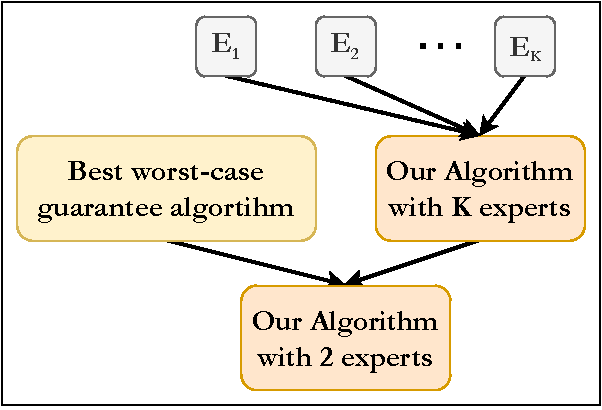
\includegraphics[width=\textwidth]{./Img/algo_mini.pdf}
			\vspace{-0.35cm}
			%\caption{Overview of the algorithm's components.}
			\label{fig:algo-layers}
	\end{minipage}

	\noindent petitive with both the \texttt{LIN-COMB} and the worst-case benchmarks,
	we proceed as follows. (The figure %\cref{fig:algo-layers}
	serves as an illustration in which  $E_1,\ \dots,\ E_K$ correspond to the online problem's experts.)
	We first apply the main algorithm on the $K$ experts' predictions to obtain an online algorithm, named $A$.
	Algorithm $A$ is $O(\ln (K))$-competitive with the \texttt{LIN-COMB} benchmark. Let $B$ be the algorithm with the best worst-case guarantee.
	We apply the main algorithm one more time on two algorithms, $A$ and $B$. The final algorithm is $O(\ln (2))$-competitive with both $A$ and $B$.
	In other words, its performance is $O(\ln (K))$-competitive with the \texttt{LIN-COMB} benchmark and is up to a constant factor worse than the best guarantee in the worst-case benchmark.
\end{proof}

